\documentclass[a4paper]{jsarticle}

\usepackage[utf8]{inputenc}

\usepackage[dvipdfmx]{graphicx}
\usepackage[dvipdfmx]{xcolor}

\usepackage{hyperref}
\usepackage{mathtools}
\usepackage{amsmath}
\usepackage{amssymb}
\usepackage{amsfonts}
\usepackage{latexsym}
\usepackage{enumitem}
\usepackage{empheq}
\usepackage{amsthm}
\usepackage{bm}
\usepackage{physics}

\begin{document}

能動的推論へのアプローチ\;:\;王道と常道
\begin{figure}[htbp]
   \centering
   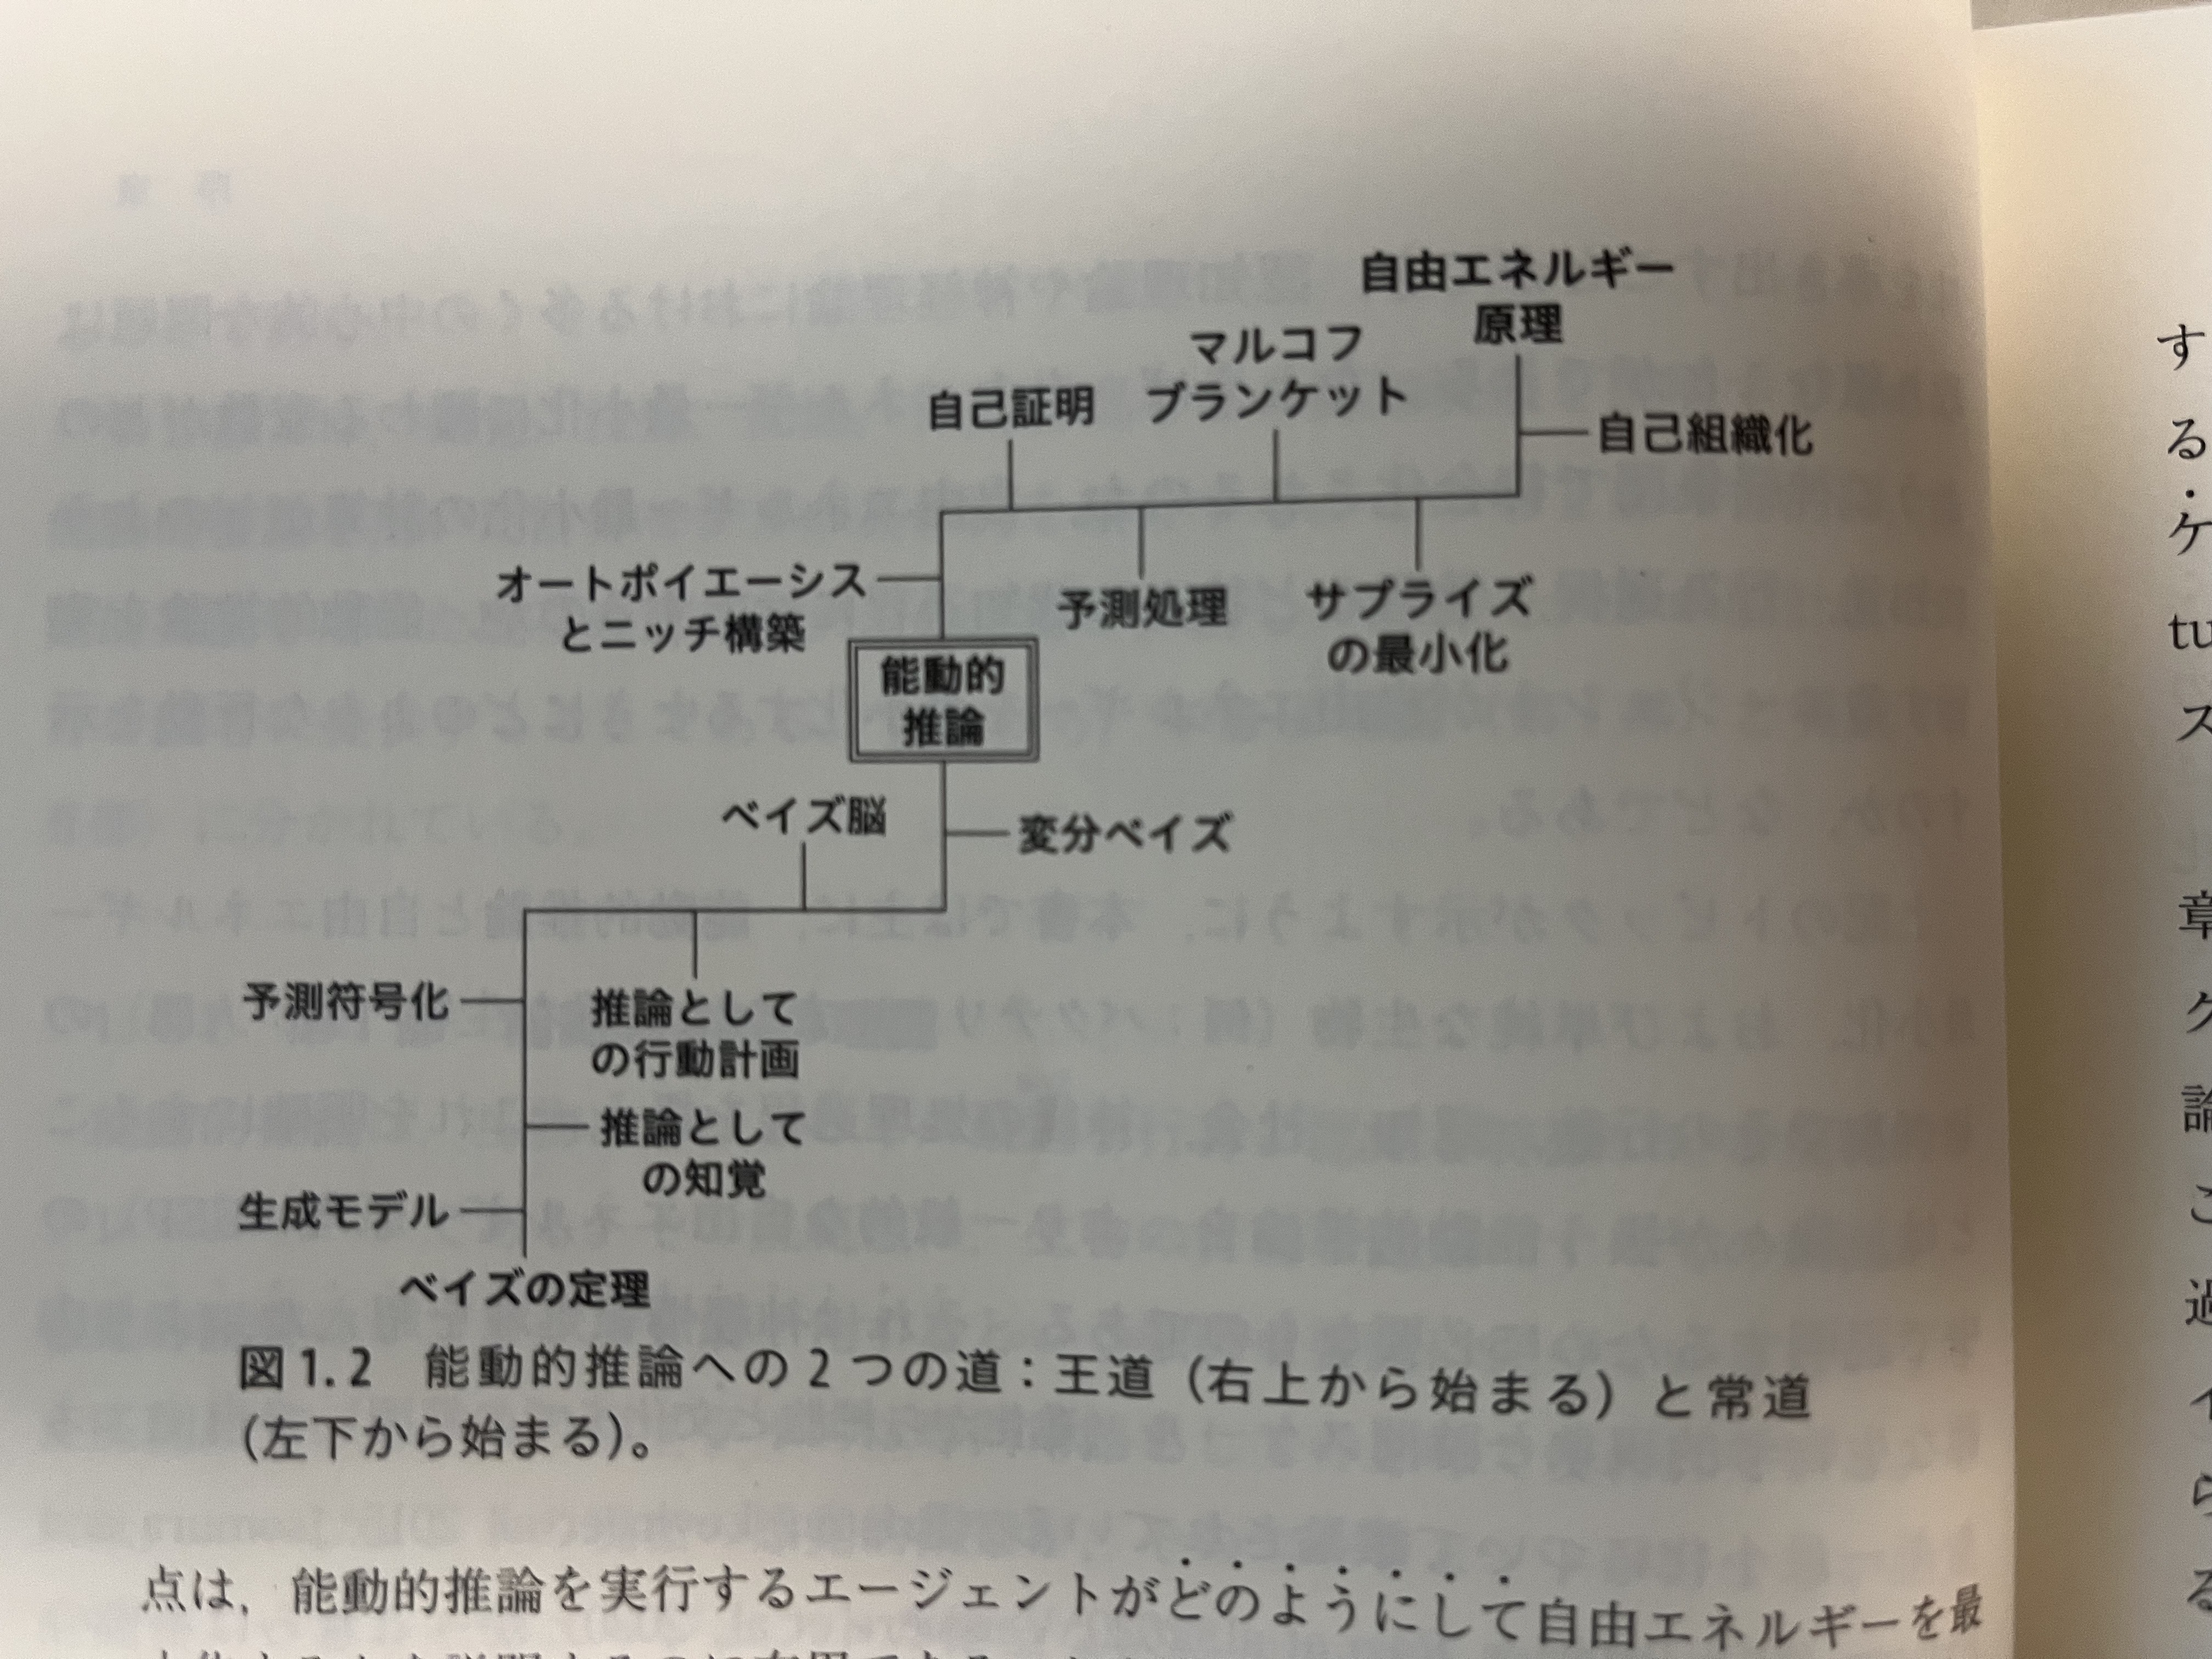
\includegraphics[scale=0.13]{approachtoAI.jpg}
\end{figure}

\section{能動的推論への常道}
ベイズ推定には生成モデルが必要である.生成モデルは観測データ$y$と,この観測データを生成する外界における生成過程内の隠れ状態$x$の,同時確率$P\qty(y,x)$として定式化される.これを
\begin{equation}
    P\qty(y,x)=P(x)P\qty(y|x)
\end{equation}
と分解すれば,2つの状態が現れる.$P\qty(x)$を事前確率といい,観測データを受け取る前の外界の隠れ状態について生物が持つ知識を表す.$P\qty(y|x)$は尤度と言い,隠れ状態からどのように観測データが生成されるかについての生物が持つ知識を示す.事前確率$P\qty(x)$から事後確率$P\qty(x|y)$を求めるには,ベイズの定理
\begin{equation}
    P(x|y)=\frac{P\qty(x)P\qty(y|x)}{P\qty(y)}
\end{equation}
を用いれば計算できる.ここで,2つのサプライズについて論ずる.1つ目は説明しようとしている感覚入力に対して,生成モデルがどれだけ適合しないかを示す指標である.このサプライズは観測データ$y$の負の対数確率
\begin{equation}
    -\ln P\qty(y)
\end{equation}
で計算される.

\end{document}